\chapter{Analytická část}\label{chap:anal}

V této kapitole se budu věnovat analýze aktuálního stavu testovací knihovny a možnostech jejího rozšíření.


\section{Analýza stávajícího stavu knihovny}

Původní testovací knihovna byla výstupem mojí bakalářské práce\cite{bakalarka} dokončené v roce 2021. Cílem této knihovny byla automatizace testů verifikace průmyslové komunikace a integrace do kontinuálního testování na Azure DevOps serveru. 

Knihovna rozlišuje tři druhy účastníků testování:

\begin{description}
    \item[Testovací služba] Služba, která řídí testovací běh.
    \item[Testované zařízení] Hlavní účastník testování, který běží na jiném zařízení, než ze kterého běží testovací služba. 
    \item[Testovací partner] Zařízení, které simuluje nějaké testované zařízení. Toto zařízení běží na stejném zařízení, jako testovací služba. 
\end{description}

Ideou knihovny je, že testovací služba, která řídí a synchronizuje běh na všech zúčastněných zařízení, je spouštěna automatizovaně za pomoci Azure DevOps serveru v Azure Pipelines. Společně s ním je spuštěn i vyvíjený produkt, který je hlavním cílem testování, v tomto kontextu nazýván jako testované zařízení. Testované zařízení se následně připojí k testovací službě a po úspěchu této fáze započne samotné testování. Implicitně knihovna tedy vyžaduje alespoň jedno nevirtualizované testované zařízení (v tomto smyslu zařízení nesmí být virtualizované testovací knihovnou). 

Pro každý test lze definovat další účastníky testování - testovací partnery. Tito testovací partneři běží pouze po dobu daného testu a po dokončení testu zaniknou. Hlavní úlohou těchto zařízení je simulace protistrany při komunikaci. 

Ukázka možného propojení všech účastníků testování je vidět na obrázku \ref{fig:bp_devicemodel}. Jak je vidět, testovací partneři a testovací služba běží na jednom zařízení, takzvaném agentovi, na kterém je primárně spouštěno celé testování. Vlevo dole je vidět testované zařízení, v tomto případě SIMATIC ET 200SP, které je propojeno s agentem. Vpravo dole můžeme vidět PLC, které pouze znázorňuje možnost propojení s dalšími externími zařízeními.

\begin{figure}[htbp]
    \centering 
    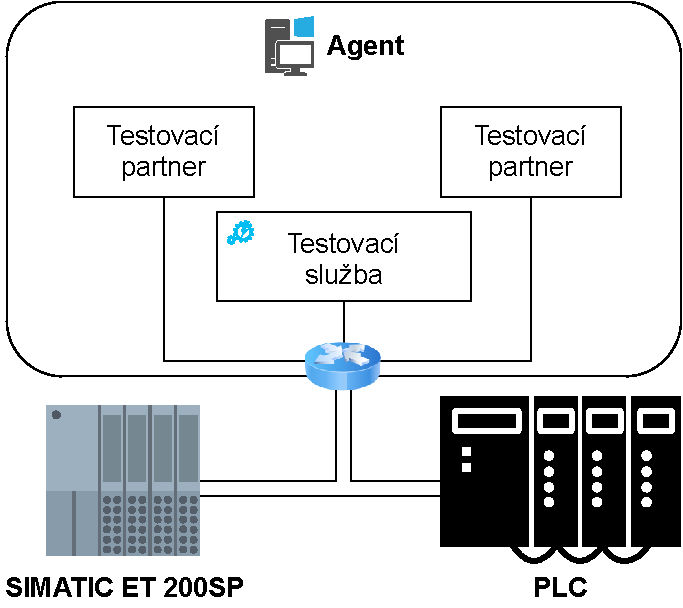
\includegraphics[width=0.97\textwidth]{assets/img/bp_assets/devicemodel.pdf}
    \caption{Ukázka možného propojení účastníků testování v původní knihovně}
    \source{Převzato z \cite{bakalarka}}
    \label{fig:bp_devicemodel}
\end{figure}


\subsection{Integrace do testovaného zařízení}

K tomu aby mohla být knihovna použita na zařízení, které je testováno, je zapotřebí nejdříve implementovat rozhraní pro testované zařízení. Implementací rozhraní jsou definovány primárně všechny potřebné funkce pro vytvoření spojení mezi testovaným zařízením a testovací službou. Zároveň definujeme funkci pro získávání instancí jednotlivých testů. 

Tyto testy rovněž dodržují jednotnou podobu pomocí rozhraní testu. Toto rozhraní definuje tři fáze testu:

\begin{enumerate}
    \item Příprava na testování -- definování potřebných struktur, inicializace.
    \item Testování -- provedení samotného testu.
    \item Úklid po testu -- uvolnění využitých zdrojů a uvedení zařízení do původního stavu.
\end{enumerate}

Všichni účastníci testu musí mít pro provedení daného testu obsahovat implementaci daného testu, definovanou rozhraním pro test, a musí být na základě obdržení identifikátoru testu schopni test instanciovat. To se provede registrací testu ve funkci \inlinecode{getTest}, která je definována rozhraním pro zařízení.

Testovací služba následně synchronizuje všechny účastníky, tak aby před započetím další testovací fáze všechna zařízení dokončila fázi předchozí. 

\subsection{Možnosti virtualizace v knihovně}

Původní testovací knihovna definuje již předem zmíněné testovací partnery, kteří jsou virtualizovaní participanti testů, sloužící k simulaci protistrany při testování průmyslové komunikace s testovaným zařízením. Jejich implementace kopíruje implementaci pro testované zařízení. Výhodou je, že k jejich využití je potřeba implementovat pouze samotné rozhraní pro test.

Každý testovací partner má životnost pouze v průběhu testu. To znamená, že před započetím testu je každý testovací partner vytvořen a připojen k testovací službě a následně po dokončení testu ukončen. Toto umožňuju variabilní počet testovacích partnerů pro každý testů.

\subsection{Topologie zapojení účastníků testu}

V případě verifikace průmyslové komunikace je samozřejmě podstatné, aby všichni účastníci testu byli schopni komunikovat mezi sebou dle potřeb daných testů. Aktuální knihovna ale toto nijak nekontroluje. 

Jediný požadavek knihovny je, aby každý účastník testu byl připojen k testovací službě a odpovídal na její požadavky. Samotné testované zařízení se připojuje před započetím testování a do konce všech testů připojeno. Testovací partneři, jak už jsem zmínil, se připojují dle potřeby před započetím jednotlivých testů.

Knihovna tedy nijak neřeší topologii zapojení jednotlivých zařízení. Je zde tedy předpoklad, že testovací partneři budou schopni komunikovat s ostatními účastníky testu díky tomu, že samotná testovací služba je schopna s nimi komunikovat. Zároveň, pokud by z nějakého důvodu komunikace nebyla možná, tak musí selhat samotné testy.

\subsection{Souhrn}

I když testovací knihovna přináší zjednodušení a automatizovaní testování průmyslové komunikace, tak stále je zde prostor pro zlepšení. Knihovna v aktuální podobě podporuje pouze limitovanou virtualizaci. Za pomoci knihovny jsme sice schopni simulovat protistranu, ale již ne samotné zařízení a to vždy musí běžet nezávisle na knihovně. 

Aktuální nový požadavek na řešení topologie zapojení zařízení nesplňuje vůbec. Zároveň je limitující požadavek, že pro každý test musí každý účastník testu obsahovat implementaci testu. Toto nemusí být vždy potřeba, například při testování veřejného rozhraní.

\section{Možnosti rozšíření virtualizačních prvků}

Z analýzy stávajícího stavu knihovny je vidět, že možnost virtualizace prostřednictvím stávající knihovny jsou limitované. Knihovna nepodporuje možnost simulovat jakékoliv zařízení a vůbec neřeší topologii zapojení daných zařízení. Rozšířením knihovny tedy chceme docílit větší možnosti virtualizace a simulace reálného prostředí. Nová knihovna by tedy měla cílit na

\begin{itemize}
    \item možnost spustit jakékoliv zařízení jako virtualizované,
    \item zapojit tato zařízení dle definované topologie (sériové linky, kruhu, hvězdy).
\end{itemize}


\subsection{Virtualizace zařízení}

Při virtualizaci zařízení máme na výběr více možností jak virtualizovat. První možnost je vytvoření virtuální mašiny pro každé zařízení prostřednictvím hypervizoru. Tato možnost sice splňuje podmínku na to spustit každé zařízení jako virtualizované, ale pro toto použití je nevhodné. 

Logickou možností je použití virtualizace skrz kontejnerizaci. Díky kontejnerizaci můžeme jednoduše spustit $n$ zařízení na jednom hardwaru. Pokud bychom měli virtuální mašiny pro $n$ zařízení, tak by zároveň muselo běžet $n$ operačních systémů, což snižuje efektivnost využití výpočetních zdrojů. Zároveň můžeme jednoduše a dynamicky vytvářet virtuální sítě, které budou splňovat požadovanou topologii. 

Toto potvrzují studie, které zkoumaly rozdíl ve výkonu a efektivnosti využití výpočetních zdrojů mezi kontejnerizací prostřednictvím softwaru Docker a virtualizačního řešení KVM, který umožnuje jádru fungovat jako hypervizor. Při jejich porovnání bylo zjištěno, že díky nástroji Docker jsou virtuální zařízení schopna být spuštěna rychleji a využívají méně výpočetních zdrojů. V porovnání při počítání HPC(High performance counting) úkolů, bylo dosaženo díky nástroji Docker lepšího výkonu o 42\,\% při úkolech náročných na procesor a o 14,98\,\% lepšího výkonu při úkolech náročných na interní paměť.\cite{kvmdockercomp}\cite{2021virt} \note{Asi bude potřebovat ještě uhladit v závuslosti na teoretické časti atd.}


\subsection{Porovnání kontejnerizačních řešení}

V dnešní době existuje mnoho řešení, který využívají kontejnerizaci. V následující sekci porovnám vybraná řešení a zhodnotím jejich vhodnost použití v testovací knihovně. 

K výběru je ale nejdříve potřeba nadefinovat úrovně správy, tedy oblasti, které můžou jednotlivé nástroje spravovat. Ty můžeme dle Aleksic\cite{docker_alt_23} rozdělit do čtyř kategorií:

\begin{description}
    \item[Image builders] Nástroje, které umožňují vytvářet kontejnery v souladu s pravidly dle OCI.
    \item[Container managers] V širším smyslu tak můžeme nazvat všechny nástroje, které pomáhají se sestavováním a během kontejnerů. Specificky ale tak můžeme nazvat ty nástroje, které pomáhají spravovat jednotlivé instance kontejnerů.
    \item[Container runtimes] Nástroje, které se starají o běh kontejnerů.
    \item[Container engines] Nástroje, které se starají o všechny procesy spojené s  kontejnerizací.
\end{description}

K úspěšnému využití kontejnerizace je samozřejmě potřeba spravovat všechny procesy spojené s kontejnerizací. Mým cílem je tedy primárně použít k řešení kontejnerizace tzv. \textit{container engines}. Jejich přímým využitím, oproti využití několika nástrojů, které by dohromady tvořili container engine, doufám předejití problémům s kompatibilitou a integrací těchto nástrojů dohromady.

Hlavním požadavkem na dané řešení je, aby podporovalo operační systém Windows. Tento požadavek primárně vyvstává z infrastruktury firmy Siemens. Vybranými řešeními tedy jsou

\begin{itemize}
    \item Docker,
    \item Podman,
    \item Vagrant. 
\end{itemize}

\subsubsection{Docker} \customtodo{zmínit docker compose a dockefile}
Docker je dle mě neznámějším a nejrozšířenějším nástrojem, který zprostředkovává kontejnerizaci. Proto také ve většině případech je většina ostatních nástrojů s Docker srovnávaná. Docker se skládá z několika hlavních komponent, které dohromady tvoří námi požadovaný container engine. Mezi tyto komponenty patří

\begin{itemize}
    \item Docker Client and Server,
    \item Docker Containers,
    \item Docker Images,
    \item Docker Registries.
\end{itemize}

Docker Client and Server jak z překladu názvu vyplývá obsahuje klienta a server. Server dostává žádosti od klienta, které následně zpracovává. Architekturu nástroje Docker můžeme vidět na obrázku \ref{fig:docker_arch}. Zajímavou komponentou je Docker Daemon, což je persistentní proces, který neustále běží na pozadí. Klient provádí komunikaci s Docker Daemon prostřednictvím stanového REST API a ten se následovně stará o sestavování, běh a distribuci Docker kontejnerů. Docker server a klient může běžet na jednom stroji, ale zároveň klient se může k serveru připojit i vzdáleně. 
\cite{turnbull2014docker}\cite{docker_overview}

\begin{figure}[htbp]
    \centering 
    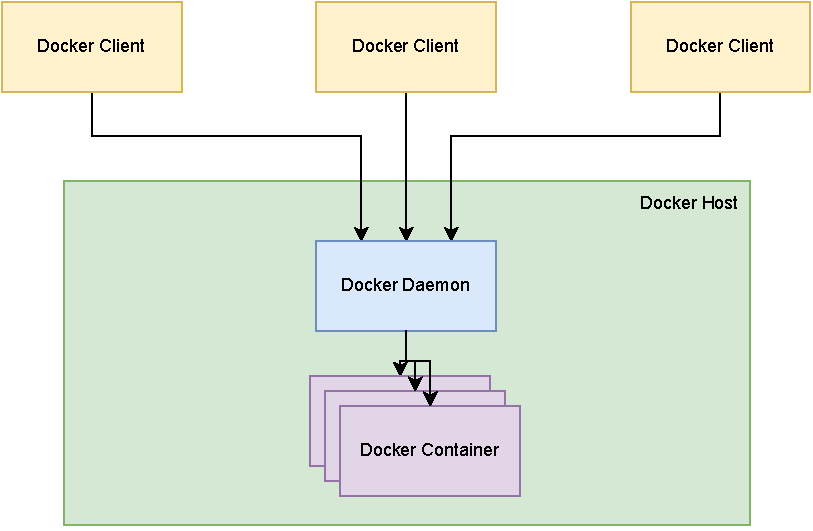
\includegraphics[width=0.97\textwidth]{assets/img/docker_arch.pdf}
    \caption{Docker architektura}
    \source{Vytvořeno dle předlohy z \cite{turnbull2014docker}}
    \label{fig:docker_arch}
\end{figure}

Jednotlivé Docker kontejnery jsou vytvářeny z tzv. Docker Images. Tyto images, neboli v češtině obrazy, obsahují definici všech závislostí a balíčků, potřebných k běhu kontejneru. Způsoby jak vytvářet obrazy jsou dva - buď můžeme definovat vlastní obraz a nebo použít nějakou již vytvořenou předlohu. Je podstatné zmínit, že každý existující obraz může být předlohou pro nový obraz. 

Tyto obrazy následně můžou být uloženy v Docker Registries. Ten slouží jako repositář pro obrazy, který může být buď veřejný, nebo soukromý. Veřejný repositář se nazývá Docker Hub, kde každý může získat kterýkoliv již vytvořený image, a nebo může také nahrát vlastní. \cite{turnbull2014docker} 

Docker v základu nabízí několik druhů síťových ovladačů. Síťový typ \textit{host} umožňuje odstranit izolaci mezi kontejnery a plně využít síť zprostředkovanou hostem, tedy Docker serverem. Oproti tomu síťový typ \textit{overlay} slouží k propojení různých Docker daemonů a umožňuje komunikace mezi nimi. 

Pro naše použití ale začínají být zajímavé až síťové typy \textit{bridge}, \textit{IPvlan} a \textit{MACvlan}. \textit{Bridge} je výchozím síťovým typem, který Docker používá v momentě kdy dva kontejnery potřebují mezi sebou komunikovat na stejném zařízení. \textit{IPvlan} oproti tomu umožňuje uživatelům plnou kontrolu nad IPv4 a IPv6 adresováním a nad druhou a třetí úrovní ISO/OSI modelu. V neposlední řadě \textit{MACvlan} umožňuje kontejnerům přiřadit různé MAC adresy, které tak mohou být odlišné od hostujícího zařízení. To umožňuje kontejnerům vypadat na síti jako fyzické zařízení.

Docker také podporuje vlastní implementace síťových ovladačů. Ty následně mohou být nahrány do stejného repositáře jako Docker obrazy. Bohužel jelikož tyto síťové ovladače jsou zahrnuty do širší kategorie \uv{rozšíření}, tak jejich vyhledávání je náročné a často neobsahují skoro žádný popis. \cite{docker_networking_overview}\cite{docker_brige_overview}

Díky tak širokému využití Docker je jeho podpora rozšířena i pro jazyk \csharp~díky knihovnám, které byly vytvořeny komunitou. Ty umožňují přímo sestavovat a nasazovat kontejnery a spravovat virtuální síť. To velice ulehčuje jeho možné použití v testovací knihovně. 

\subsubsection{Podman}
Podman je velice podobný Dockeru. Tento nástroj je primárně zaměřený na operační systém Linux, kde pomáhá najít, spustit a nasadit kontejnery dle pravidel OCI. V použití je dokonce až tak podobný, že většina uživatelů může změnit příkaz \inlinecode{docker} na \inlinecode{podman} bez problémů. Rozdíly tam ale přeci jen jsou. 

Podman oproti Docker používá takzvanou \textit{daemon-less} architekturu. Jak už bylo zmíněno, Docker obsahuje neustále běžící proces který se nazývá \textit{daemon}, který poslouchá příkazy od klienta a spravuje všechny procesy spojené s kontejnerizací. Tento přístup vytváří problémy hlavně z bezpečnostního hlediska, jelikož daemon musí být spuštěn s právy správce počítače. Docker sice podporuje od verze v19.03 tzv. \textit{rootless execution}, tedy mód kdy nepotřebuje práva správce, ale při chodu v tomto módu mohou uživatelé narazit na různé limitace.

A na toto se přesně zaměřil Podman. Podman používá pro správu kontejnerů nástroj \textit{systemd}, který ke spuštění využívá práva uživatele, který provádí příkazy. Podman také využívá jiný nástroj \textit{Buildah}, za pomocí něhož je schopen sestavovat kontejnery bez daemona. \cite{podman}\cite{podman_vs_docker}

Podman stejně jako Docker podporuje síťové typy \textit{bridge} a \textit{MACvlan}. Ovšem k jejich použití již potřebuje práva správce počítače. K vyřešení tohoto problému Podman používá síťový typ \textit{slirp4netns}. Ta vytvoří speciální TAP zařízení, fungující na linkové vrstvě ISO/OSI modelu a umožňuje komunikaci mezi kontejnery, které jsou ovšem takto fungují izolovaně od sebe. \cite{podman_network}

Jak jsem řekl na začátku, Podman je nástroj primárně zaměřený na operační systém Linux, ovšem má i svou distribuci pro Windows. Ovšem k tomu aby mohl na Windows fungovat, tak každý kontejner musí obsahovat hostující systém Linux, na kterém jsou následně kontejnery spuštěny. \cite{podman_vs_docker}

\subsubsection{Vagrant}

Vagrant je nástroj, který se primárně zaměřuje na to, aby přinesl konzistentní vývojové prostředí na různé operační systémy. Jeho hlavní výhodou oproti Docker je jeho široká podpora operačních systému, které Docker nepodporuje. 

Stejně jako Docker, i Vagrant má širokou podporu komunitních obrazů, ze kterých jsou následně vytvářeny tzv. \textit{boxy}, což je pouze jiný název pro kontejnery.\cite{vargrant_vs_docker}
\customtodo{Rozšířit}

V některých aspektech jsou ovšem ostatní možnosti lepší volbou. Jednou z nich je využití výpočetních zdrojů. Oproti Docker, který používá přímo zdroje hostujícího stroje, tak každá virtuální mašina vytvořená ve Vagrant spotřebuje specifický počet jáder, paměti RAM a paměti na disku. Zároveň čas změny konfigurace a sestavení virtuální mašiny je mnohem rychlejší na Docker, než ve Vagrant.\cite{madapparambath_2022}
\question{Nechat Vagrant nebo ne, jelikož co koukám tak to kontejnerizaci nedělá? Hledat náhradu?}

\subsection{Shrnutí}

Při pohledu na vytvořenou analýzu je vidět, že Vagrant vyšel z této analýzy na poslední příčce. Díky rozdílnému primárnímu zaměření pokulhává v několika kategoriích, především v efektivitě využití výpočetních zdrojů. Zároveň za tuto velkou cenu nepřináší žádné výhody oproti ostatním nástrojům.

Docker a Podman jsou velice podobné nástroje a ve spoustě případů je každý z nich dobrou volbou. Pro použití v testovací knihovně ovšem vyhrává Docker. Hlavním důvodem je jeho nativní podpora platformy Windows. Další velkou výhodou je jeho široká rozšířenost, což vede k velice aktivní komunitě vývojářů, jejichž knihovny a návody velice usnadňují jeho integraci. 